% Document setup
\documentclass[12pt]{article}
\usepackage[margin=1in]{geometry}
\usepackage{fancyhdr}
\usepackage{lastpage}

\pagestyle{fancy}
\lhead{Richard Whitehill}
\chead{PHYS 804 -- HW \HWnum}
\rhead{\duedate}
\cfoot{\thepage \hspace{1pt} of \pageref{LastPage}}

% Encoding
\usepackage[utf8]{inputenc}
\usepackage[T1]{fontenc}

% Math/Physics Packages
\usepackage{amsmath}
\usepackage{amssymb}
\usepackage{mathtools}
\usepackage{physics}
\usepackage{siunitx}

\AtBeginDocument{\RenewCommandCopy\qty\SI}

% Enumeration/itemize
\usepackage{enumitem}
\newenvironment{parts}
{\begin{enumerate}[label=\textbf{(\alph*)},leftmargin=*,itemsep=-10pt]
}{\end{enumerate}}

% Reference Style
\usepackage{hyperref}
\hypersetup{
    colorlinks=true,
    linkcolor=blue,
    filecolor=magenta,
    urlcolor=cyan,
    citecolor=green
}

\newcommand{\eref}[1]{Eq.~(\ref{eq:#1})}
\newcommand{\erefs}[2]{Eqs.~(\ref{eq:#1})--(\ref{eq:#2})}

\newcommand{\fref}[1]{Fig.~\ref{fig:#1}}
\newcommand{\frefs}[2]{Figs.~\ref{fig:#1}--\ref{fig:#2}}

\newcommand{\tref}[1]{Table~\ref{tab:#1}}
\newcommand{\trefs}[2]{Tables~\ref{tab:#1}-\ref{tab:#2}}

% Figures and Tables 
\usepackage{graphicx}
\usepackage{float}
\usepackage[font=small,labelfont=bf]{caption}

\newcommand{\bef}{\begin{figure}[h!]\begin{center}}
\newcommand{\eef}{\end{center}\end{figure}}

\newcommand{\bet}{\begin{table}[h!]\begin{center}}
\newcommand{\eet}{\end{center}\end{table}}

% tikz
\usepackage{tikz}
\usetikzlibrary{calc}
\usetikzlibrary{decorations.pathmorphing}
\usetikzlibrary{decorations.markings}
\usetikzlibrary{arrows.meta}
\usetikzlibrary{positioning}
\usetikzlibrary{3d}
\usetikzlibrary{shapes.geometric}

% tcolorbox
\usepackage[most]{tcolorbox}
\usepackage{xcolor}
\usepackage{xifthen}
\usepackage{parskip}

\newcommand*{\eqbox}{\tcboxmath[
    enhanced,
    colback=black!10!white,
    colframe=black,
    sharp corners,
    size=fbox,
    boxsep=8pt,
    boxrule=1pt
]}

% problem-solution macros
% \usepackage{adjustbox}
\usepackage{changepage}

\newtcolorbox{probbox}[1][]{
    breakable,
    enhanced,
    boxrule=0pt,
    frame hidden,
    borderline west={4pt}{0pt}{green!50!black},
    colback=green!5,
    before upper=\textbf{Problem #1) \,},
    % \textbf{Problem #1 \ifthenelse{\isempty{#1}}{}{: #1} \\ },
    sharp corners,
    parbox=false
}

% \newtcolorbox{ProblemBox}[1][]{%
%   breakable,
%   enhanced,
%   colback=black!10!white,
%   colframe=black,
%   title={\large #1 \hfill}
% }
\newcommand{\prob}[2]{
\begin{probbox}[#1]
#2
\end{probbox}
}

\newenvironment{solution}{\begin{adjustwidth}{8pt}{8pt}}{\end{adjustwidth}}
\newcommand{\sol}[1]{
\begin{solution}
#1
\end{solution}
}
% \textbf{#1)} #2}

% Miscellaneous Definitions/Settings
\newcommand{\reals}{\mathbb{R}}
\newcommand{\integers}{\mathbb{Z}}
\newcommand{\naturals}{\mathbb{N}}
\newcommand{\rationals}{\mathbb{Q}}
\newcommand{\complexs}{\mathbb{C}}

\setlength{\parskip}{\baselineskip}
\setlength{\parindent}{0pt}
\setlength{\headheight}{14.49998pt}
\addtolength{\topmargin}{-2.49998pt}


\def\HWnum{5}
\def\duedate{October 17, 2024}

\begin{document}

\prob{1}{

Consider again the classical complex Klein-Gordon field with the Lagrangian density
\begin{align}
    \mathcal{L} = ( \partial_{\mu} \phi ) ( \partial^{\mu} \phi^{*} ) - m^2 \phi \phi^{*}
.\end{align}
Repeat and write out all the steps that I showed in class for converting a real, lattice Klein-Gordon field to a quantum continuum version, but now for the complex scalar field above.
Get the Heisenberg field operators $\hat{\phi}(x)$ and $\hat{\phi}^{\dagger}$ in terms of the creation and annihilation operators for particles and antiparticles.

}

\sol{

In this problem, we can introduce some system with complex generalized coordinates $q_{\vb*{n}}$ as in HW 4, problem 3 governed by a Lagrangian
\begin{align}
    L = \sum_{\vb*{n}} \frac{1}{2} |\dot{q}_{\vb*{n}}|^2 - \sum_{\vb*{n}} \frac{m^2}{2} |q_{\vb*{n}}|^2 - \sum_{\vb*{n}} \sum_{i} \frac{\kappa}{2} |q_{\vb*{n} + \vu*{e}_{i}} - q_{\vb*{n}}|^2
.\end{align}
Notice that we can write this in terms of the real and imaginary parts of $q_{\vb*{n}}$.
For brevity, let us adopt notation where $\Re(q_{n}) = q_{R,\vb*{n}}$ and $\Im(q_{\vb*{n}}) = q_{I,\vb*{n}}$
\begin{align}
    L &= \sum_{\vb*{n}} \Bigg\{ \frac{1}{2} \dot{q}_{R,\vb*{n}}^2 - \frac{m^2}{2} q_{\vb*{R,\vb*{n}}}^2 - \frac{\kappa}{2} [ q_{R,\vb*{n} + \vu*{e}_{i}} - q_{R,\vb*{n}} ]^2 \Bigg\} \nonumber \\
      &+ \sum_{\vb*{n}} \Bigg\{ \frac{1}{2} \dot{q}_{I,\vb*{n}}^2 - \frac{m^2}{2} q_{\vb*{I,\vb*{n}}}^2 - \frac{\kappa}{2} [ q_{I,\vb*{n} + \vu*{e}_{i}} - q_{I,\vb*{n}} ]^2 \Bigg\}
.\end{align}
Hence, we can treat the real and imaginary parts as separate real-valued generalized coordinates and carry over the treatment from the prior homework and lectures.
We therefore find that the conjugate momenta to the real and imaginary parts of $q_{\vb*{n}}$ are
\begin{align}
    p_{R,\vb*{n}} = \dot{q}_{R,\vb*{n}}, \quad p_{I,\vb*{n}} = \dot{q}_{I,\vb*{n}}
,\end{align}
respectively.
Beware: it is tempting to conflate $p_{R,\vb*{n}}$ and $p_{I,\vb*{n}}$ with the real and imaginary parts of the complex generalized momentum $p_{\vb*{n}}$ conjugate to $q_{\vb*{n}}$, but this is not exactly the case since
\begin{align}
    p_{\vb*{n}} = \pdv{L}{\dot{q}_{\vb*{n}}} = \frac{1}{2} \Bigg( \pdv{L}{\dot{q}_{R,\vb*{n}}} - i \pdv{L}{\dot{q}_{I,\vb*{n}}} \Bigg) = \frac{1}{2} ( p_{R,\vb*{n}} - i p_{I,\vb*{n}} ) = \frac{1}{2} \dot{q}_{\vb*{n}}^{*}
.\end{align}
In terms of these momenta and coordinates, we find
\begin{align}
    H &= \sum_{\vb*{n}} \Bigg\{ \frac{1}{2} p_{R,\vb*{n}}^2 - \frac{m^2}{2} q_{R,\vb*{n}}^2 - \frac{\kappa}{2} [q_{R,\vb*{n} + \vu*{e}_{i}} - q_{R,\vb*{n}}]^2  \Bigg\} \nonumber \\
    &+ \sum_{\vb*{n}} \Bigg\{ \frac{1}{2} p_{I,\vb*{n}}^2 - \frac{m^2}{2} q_{I,\vb*{n}}^2 - \frac{\kappa}{2} [q_{I,\vb*{n} + \vu*{e}_{i}} - q_{I,\vb*{n}}]^2  \Bigg\}
.\end{align}
At this point, normal coordinates are introduced such that
\begin{align}
    q_{R/I,\vb*{n}} &= \frac{1}{N^{D/2}} \sum_{\vb*{k}} \bar{q}_{R/I,\vb*{k}} e^{i a \vb*{k} \cdot \vb*{n}} \\
    p_{R/I,\vb*{n}} &= \frac{1}{N^{D/2}} \sum_{\vb*{k}} \bar{p}_{R/I,\vb*{k}} e^{i a \vb*{k} \cdot \vb*{n}}
,\end{align}
and the imposition of periodic boundary conditions in our finite space of volume $L^{D}$ gives
\begin{align}
    \vb*{k} = \frac{2 \pi \bar{\vb*{n}}}{L}
,\end{align}
with the components of our reciprocal lattice vector $\bar{n}_{i} \in (-N/2,N/2]$.
Additionally, imposing the realness of our coordinates and momenta gives that
\begin{align}
    \bar{q}_{R/I,\vb*{k}}^{*} = \bar{q}_{R/I,-\vb*{k}}, \quad \bar{q}_{R/I,\vb*{k}}^{*} = \bar{p}_{R/I,-\vb*{k}}
.\end{align}
Thus, using all the machinery built up in the previous homeworks and lectures, we find that
\begin{align}
    H &= \sum_{\vb*{k}} \Bigg\{ \frac{1}{2} \bar{p}_{R,\vb*{k}} \bar{p}_{R,-\vb*{k}} + \frac{\omega_{\vb*{k}}^2}{2} \bar{q}_{R,\vb*{k}} \bar{q}_{R,-\vb*{k}} \Bigg\} \nonumber \\
    &+ \sum_{\vb*{k}} \Bigg\{ \frac{1}{2} \bar{p}_{I,\vb*{k}} \bar{p}_{I,-\vb*{k}} + \frac{\omega_{\vb*{k}}^2}{2} \bar{q}_{I,\vb*{k}} \bar{q}_{I,-\vb*{k}} \Bigg\}
,\end{align}
where
\begin{align}
    \omega_{\vb*{k}}^2 = m^2 + 2 \kappa \sum_{i} [ 1 - \cos(k_{i} a) ]
.\end{align}
Again, one can see using the realness condition that the real and imaginary parts of the $k$-modes are fully decoupled harmonic oscillators.
We then introduce the canonical commutation relations
\begin{align}
    [\bar{q}_{R/I,\vb*{k}},\bar{p}_{R/I,-\vb*{k}'}] = i \delta_{\vb*{k},\vb*{k}'}
,\end{align}
where the rest of the combinations give zero.
From this, we introduce the creation and annihilation operators $a_{R/I,\vb*{k}}^{\dagger}$ and $a_{R/I,\vb*{k}}$, respectively, such that
\begin{align}
    \bar{q}_{R/I,\vb*{k}} = \frac{1}{\sqrt{2 \omega_{\vb*{k}}}} ( a_{R/I,\vb*{k}} + a_{R/I,-\vb*{k}}^{\dagger} ) \\
    \bar{p}_{R/I,\vb*{k}} = -i \sqrt{\frac{\omega_{\vb*{k}}}{2}} ( a_{R/I,\vb*{k}} - a_{R/I,-\vb*{k}}^{\dagger} )
.\end{align}
Observe then that the creation and annihilation satisfy the typical commutation relations:
\begin{align}
    [a_{R/I,\vb*{k}},a_{R/I,\vb*{k}'}^{\dagger}] = \delta_{\vb*{k},\vb*{k}'}
,\end{align}
and thus, the Hamiltonian can be expressed as
\begin{align}
    H = \sum_{\vb*{k}} \omega_{\vb*{k}} \Big( a_{R,\vb*{k}}^{\dagger} a_{R,\vb*{k}} + a_{I,\vb*{k}}^{\dagger} a_{I,\vb*{k}} + 1 \Big)
.\end{align}
At this point, we would like to translate our results to complex coordinates and momenta.
In terms of the real and imaginary parts, we have
\begin{align}
    q_{\vb*{n}} = \frac{1}{N^{D/2}} \sum_{\vb*{k}} (\bar{q}_{R,\vb*{k}} + i \bar{q}_{I,\vb*{k}}) e^{i a \vb*{k} \cdot \vb*{n}} = \frac{1}{N^{D/2}} \sum_{\vb*{k}} \bar{q}_{\vb*{k}} e^{i a \vb*{k} \cdot \vb*{n}} \nonumber \\
    p_{\vb*{n}} = \frac{1}{N^{D/2}} \sum_{\vb*{k}} \frac{1}{2} ( \bar{p}_{R,\vb*{k}} - i p_{I,\vb*{k}} ) e^{i a \vb*{k} \cdot \vb*{n}} = \frac{1}{N^{D/2}} \sum_{\vb*{k}} \bar{p}_{\vb*{k}} e^{i a \vb*{k} \cdot \vb*{n}}
.\end{align}
Observe that these redefined Fourier coefficients have the desired commutation relations:
\begin{align}
    [\bar{q}_{\vb*{k}},\bar{p}_{-\vb*{k}}] = \frac{1}{2} [q_{R,\vb*{k}} + i \bar{q}_{I,\vb*{k}}, \bar{p}_{R,-\vb*{k}} - i \bar{p}_{I,-\vb*{k}}] = i \delta_{\vb*{k}',\vb*{k}'} \\
    [\bar{q}_{\vb*{k}}^{*},\bar{p}_{-\vb*{k}}^{*}] = \frac{1}{2} [ \bar{q}_{R,\vb*{k}} - i \bar{q}_{I,\vb*{k}}, \bar{p}_{R,-\vb*{k}} + i \bar{p}_{I,-\vb*{k}} ] = i \delta_{\vb*{k},\vb*{k}'}
.\end{align}
Additionally, we have 
\begin{align}
    \bar{q}_{\vb*{k}} &= \frac{1}{\sqrt{2 \omega_{\vb*{k}}}} \Big[ ( a_{R,\vb*{k}} + i a_{I,\vb*{k}} ) + ( a_{R,-\vb*{k}}^{\dagger} + i a_{I,-\vb*{k}}^{\dagger} ) \Big] = \frac{1}{\sqrt{\omega_{\vb*{k}}}} ( a_{\vb*{k}} + b_{-\vb*{k}}^{\dagger} ) \\
    \bar{q}_{\vb*{k}}^{*} &= \frac{1}{\sqrt{2 \omega_{\vb*{k}}}} \Big[ ( a_{R,\vb*{k}} - i a_{I,\vb*{k}} ) + ( a_{R,-\vb*{k}}^{\dagger} - i a_{I,-\vb*{k}}^{\dagger} ) \Big] = \frac{1}{\sqrt{\omega_{k}}} ( b_{\vb*{k}} + a_{-\vb*{k}}^{\dagger} )
,\end{align}
Again, it is not too difficult to show that these redefined creation and annihilation operators satisfy the necessary commutation relations
\begin{align}
    [a_{\vb*{k}},a_{\vb*{k}'}^{\dagger}] = \frac{1}{2} [ a_{R,\vb*{k}} + i a_{I,\vb*{k}}, a_{R,\vb*{k}'}^{\dagger} - i a_{I,\vb*{k}'}^{\dagger} ] = \delta_{\vb*{k},\vb*{k}'} \\
    [b_{\vb*{k}},b_{\vb*{k}'}^{\dagger}] = \frac{1}{2} [ a_{R,\vb*{k}} - i a_{I,\vb*{k}}, a_{R,\vb*{k}'}^{\dagger} + i a_{I,\vb*{k}'}^{\dagger} ] = \delta_{\vb*{k},\vb*{k}'}
\end{align}
and that our Hamiltonian
\begin{align}
    H = \sum_{\vb*{k}} \omega_{\vb*{k}} ( a_{\vb*{k}}^{\dagger} a_{\vb*{k}} + b_{\vb*{k}}^{\dagger} b_{\vb*{k}} + 1 )
.\end{align}

At this point, we can go directly and write the generalized coordinates in terms of these creation and annihilation operators:
\begin{align}
    q_{\vb*{n}} &= \frac{1}{N^{D/2}} \sum_{\vb*{k}} \frac{1}{\sqrt{\omega_{\vb*{k}}}} \Big( a_{\vb*{k}} e^{i a \vb*{k} \cdot \vb*{n}} + b_{-\vb*{k}}^{\dagger} e^{i a \vb*{k} \cdot \vb*{n}} \Big) \\
    q_{\vb*{n}}^{\dagger} &= \frac{1}{N^{D/2}} \sum_{\vb*{k}} \frac{1}{\sqrt{\omega_{\vb*{k}}}} \Big( a_{\vb*{k}}^{\dagger} e^{-i a \vb*{k} \cdot \vb*{n}} + b_{-\vb*{k}} e^{-i a \vb*{k} \cdot \vb*{n}} \Big)
.\end{align}
These are the Schr\"{o}dinger picture operators, but we can change pictures using the typical prescription ($\mathcal{O}_{H} = e^{i H t} \mathcal{O}_{S} e^{-i H t}$) and the time dependence of the Heisenberg picture creation and annihilation operators (derived in HW 4 problem 2a):
\begin{align}
    q_{\vb*{n}}(t) &= \frac{1}{N^{D/2}} \sum_{\vb*{k}} \frac{1}{\sqrt{\omega_{\vb*{k}}}} \Big( a_{\vb*{k}} e^{- i \omega_{\vb*{k}} t + i a \vb*{k} \cdot \vb*{n}} + b_{\vb*{k}}^{\dagger} e^{i \omega_{\vb*{k}} t - i a \vb*{k} \cdot \vb*{n}} \Big) \nonumber \\
                   &= \frac{1}{N^{D/2}} \sum_{\vb*{k}} \frac{1}{\sqrt{\omega_{\vb*{k}}}} \Big( a_{\vb*{k}} e^{-i k \cdot x} + b_{\vb*{k}}^{\dagger} e^{i k \cdot x} \Big) \\
    q_{\vb*{n}}^{\dagger}(t) &= \frac{1}{N^{D/2}} \sum_{\vb*{k}} \frac{1}{\sqrt{\omega_{\vb*{k}}}} \Big( a_{\vb*{k}}^{\dagger} e^{i \omega_{\vb*{k}} t - i a \vb*{k} \cdot \vb*{n}} + b_{\vb*{k}} e^{-i \omega_{\vb*{k}}t + i a \vb*{k} \cdot \vb*{n}} \Big) \nonumber \\
                             &= \frac{1}{N^{D/2}} \sum_{\vb*{k}} \frac{1}{\sqrt{\omega_{\vb*{k}}}} \Big( a_{\vb*{k}}^{\dagger} e^{i k \cdot x} + b_{\vb*{k}} e^{-ik \cdot x} \Big)
.\end{align}
Finally, we take the continuum limit by first taking $a \rightarrow 0$ and $N \rightarrow \infty$, holding $L$ fixed.
Defining $\phi(\vb*{x}) = q_{\vb*{n}} / a^{D/2}$ and similarly for the complex conjugate, we have
\begin{align}
    \phi(\vb*{x}) &= \sum_{\vb*{k}} \frac{1}{L^{D/2} \sqrt{\omega_{\vb*{k}}}} \Big( a_{\vb*{k}} e^{-i k \cdot x} + b_{\vb*{k}}^{\dagger} e^{i k \cdot x} \Big) \\
    \phi^{\dagger}(\vb*{x}) &= \sum_{\vb*{k}} \frac{1}{L^{D/2} \sqrt{\omega_{\vb*{k}}}} \Big( a_{\vb*{k}}^{\dagger} e^{i k \cdot x} + b_{\vb*{k}} e^{-i k \cdot x} \Big)
.\end{align}
Next, we take the infinite volume limit via $L \rightarrow \infty$ and redefining our continuum limit creation and annihilation operators via $a_{\vb*{k}} \rightarrow a_{\vb*{k}} / L^{D/2}$ and similarly for $b_{\vb*{k}}$.
Thus,
\begin{align}
\eqbox{
\begin{aligned} 
    \phi(\vb*{x}) &= \int \frac{\dd[D]{\vb*{k}}}{(2 \pi)^{D} \sqrt{\omega_{\vb*{k}}}} \Big( a_{\vb*{k}} e^{-i k \cdot x} + b_{\vb*{k}}^{\dagger} e^{i k \cdot x} \Big) \\
    \phi^{\dagger}(\vb*{x}) &= \int \frac{\dd[D]{\vb*{k}}}{(2 \pi)^{D} \sqrt{\omega_{\vb*{k}}}} \Big( a_{\vb*{k}}^{\dagger} e^{i k \cdot x} + b_{\vb*{k}} e^{-i k \cdot x} \Big)
.\end{aligned}
}
\end{align}

}


\newpage
\prob{2}{

Checking steps from class.

\begin{parts}
   
\item Show that the effect of normal ordering on the Hamiltonian and Noether momentum is to eliminate any constant terms and puts $:\hat{H}:$ and $:\hat{P}_{j}:$ into a form that only involves number operators.

\item Verify that the expression for the identity in the Fock space that we discussed class is
    \begin{align}
        \hat{1} = \sum_{n=0}^{\infty} \frac{1}{n!} \int \prod_{j=0}^{n} \frac{\dd[3]{\vb*{p}_{j}}}{(2 \pi)^3 2 E_{\vb*{p}_{j}}} \ket{p_{n}}\bra{p_{n}}
    \end{align}
    for the case of a three-excitation momentum state $\ket{\vb*{k}_{1},\vb*{k}_{2},\vb*{k}_{3}}$.

\item As in class, let a single excitation element of a bosonic Fock space at time $t$ be
    \begin{align}
        \ket{f,1,t} = \int \frac{\dd[3]{\vb*{p}}}{(2\pi)^3 \sqrt{2 E_{\vb*{p}}}} \tilde{f}(\vb*{p}) \ket{\vb*{p}} = \int \frac{\dd[3]{\vb*{p}}}{(2 \pi)^3} a_{\vb*{p}}^{\dagger} \ket{0} \tilde{f}(\vb*{p})
    \end{align}
    with a wavepacket function $\tilde{f}(\vb*{p})$.
    Let the coordinate space wavepacket function be defined by
    \begin{align}
        f(x) = \int \frac{\dd[3]{\vb*{p}}}{(2 \pi)^3 \sqrt{2 E_{\vb*{p}}}} \tilde{f}(\vb*{p}) e^{-i p \cdot x} = \int \frac{\dd[3]{\vb*{p}}}{(2 \pi)^3 \sqrt{2 E_{\vb*{p}}}} \tilde{f}(\vb*{p}) e^{-i p^{0} t + i \vb*{p} \cdot \vb*{x}}
    .\end{align}
    Note the time dependence in the exponential despite the fact that the integral is only over spatial components.
    Show that
    \begin{align}
        \ket{f,1,t} = \int \dd[3]{\vb*{x}} \phi(\vb*{x}) \ket{0} 2 i \pdv{f(x)}{t}
    .\end{align}

\item By using Fock states expressed like in Eq. (3) above, show directly that $a_{\vb*{k}}^{\dagger} a_{\vb*{k}}$ is a density of excitations with respect to three momentum.

\end{parts}

}

\sol{

(a) For simplicity, we work in the context of a free scalar field theory (i.e. real Klein-Gordon theory).
In this theory, our energy-momentum tensor
\begin{align}
    T^{\mu\nu} = \partial^{\mu} \phi \partial^{\nu} \phi - \frac{1}{2} g^{\mu\nu} ( \partial^{\rho} \phi \partial_{\rho} \phi - m^2 \phi^2 )
.\end{align}
Thus, the 4-momentum operator
\begin{align}
    P^{\mu} = \int \dd[3]{\vb*{x}} T^{0\mu} = \int \dd[3]{\vb*{x}} \Big\{ \dot{\phi} \partial^{\mu} \phi - \frac{1}{2} g^{0 \mu} \Big( \partial^{\rho} \phi \partial_{\rho} \phi - m^2 \phi^2 \Big) \Big\}
.\end{align}
The Hamiltonian is then
\begin{align}
    H = P^{0} = \frac{1}{2} \int \dd[3]{\vb*{x}} \Bigg\{ \dot{\phi}^2 + ( \grad \phi )^2 + m^2 \phi^2 \Bigg\}
\end{align}
whilst the components of the momentum operator
\begin{align}
    P^{i} = \int \dd[3]{\vb*{x}} \dot{\phi} \partial^{i} \phi
.\end{align}
Inserting the mode expansion of $\phi$ we find
\begin{align}
\eqbox{
\begin{aligned} 
    H &= \int \frac{\dd[3]{\vb*{k}}}{(2 \pi)^3} \frac{\omega_{\vb*{k}}}{2} ( a_{\vb*{k}}^{\dagger} a_{\vb*{k}} + a_{\vb*{k}} a_{\vb*{k}}^{\dagger} ) \Rightarrow :H: = \int \frac{\dd[3]{\vb*{k}}}{(2 \pi)^3} \omega_{\vb*{k}} a_{\vb*{k}}^{\dagger} a_{\vb*{k}} \\
    P^{i} &= \int \frac{\dd[3]{\vb*{k}}}{(2 \pi)^3} \frac{k^{i}}{2} ( a_{\vb*{k}}^{\dagger} a_{\vb*{k}} + a_{\vb*{k}} a_{\vb*{k}}^{\dagger} ) \Rightarrow :P^{i}: = \int \frac{\dd[3]{\vb*{k}}}{(2 \pi)^3} k^{i} a_{\vb*{k}}^{\dagger} a_{\vb*{k}}
.\end{aligned}
}
\end{align}
It is simple to see that these normal ordered operators only contain number operators and no infinities.


(b) We verify this directly:
\begin{align}
\eqbox{
\begin{aligned} 
    \hat{1} \ket{\vb*{k}_{1},\vb*{k}_{2},\vb*{k}_{3}} &= \sum_{n=0}^{\infty} \frac{1}{n!} \int \prod_{j=0}^{n} \frac{\dd[3]{\vb*{p}_{j}}}{(2 \pi)^3 2 E_{\vb*{p}_{j}}} \ket{p_{n}} \ip{p_{n}}{\vb*{k}_{1},\vb*{k}_{2},\vb*{k}_{3}} \\
                                                      &= \sum_{n=0}^{\infty} \frac{1}{n!} \int \prod_{j=0}^{n} \frac{\dd[3]{\vb*{p}_{j}}}{(2 \pi)^3 2 E_{\vb*{p}_{j}}} \ket{\vb*{p}_{1},\vb*{p}_{2},\vb*{p}_{3}} \delta_{n 3} \sum_{\sigma \in S_{n}} \prod_{\ell} (2 \pi)^3 2 E_{\vb*{k}_{\ell}} \delta(\vb*{k}_{\ell} - \vb*{p}_{\sigma(\ell)}) \\
                                                      &= \frac{1}{3!} \sum_{\sigma \in S_{n}} \ket{\vb*{k}_{\sigma(1)},\vb*{k}_{\sigma(2)},\vb*{k}_{\sigma(3)}} = \ket{\vb*{p}_{1},\vb*{p}_{2},\vb*{p}_{3}}
.\end{aligned}
}
\end{align}


(c) We can invert the ``Fourier transform'' via the following procedure
\begin{gather}
    \int \dd[3]{\vb*{x}} f(x) e^{i p^{0} t - i \vb*{p} \cdot \vb*{x}} = \int \frac{\dd[3]{\vb*{p}'}}{(2 \pi)^3 \sqrt{2 E_{\vb*{p}'}}} \tilde{f}(\vb*{p}') \underbrace{ \int \dd[3]{\vb*{x}} e^{i ( \vb*{p} - \vb*{p}') \cdot \vb*{x}} }_{(2 \pi)^3 \delta(\vb*{p} - \vb*{p}')} = \frac{1}{\sqrt{2 E_{\vb*{p}}}} \tilde{f}(\vb*{p}) \nonumber \\
    \tilde{f}(\vb*{p}) = \int \dd[3]{\vb*{x}} \sqrt{2 E_{\vb*{p}}} e^{i p \cdot x} f(x)
.\end{gather}
Putting this into the wavepacket state
\begin{align}
    \ket{f,1,t} &= \int \frac{\dd[3]{\vb*{p}}}{(2 \pi)^3} a_{\vb*{p}}^{\dagger} \ket{0} \int \dd[3]{\vb*{x}} \sqrt{2 E_{\vb*{p}}} e^{i p \cdot x} f(\vb*{x}) \nonumber \\
                &= \int \dd[3]{\vb*{x}} f(x) \int \frac{\dd[3]{\vb*{p}}}{(2 \pi)^3 \sqrt{2 E_{\vb*{p}}}} 2 E_{\vb*{p}} a_{\vb*{p}}^{\dagger} e^{i p \cdot k} \ket{0} \nonumber \\
                &= \eqbox{ \int \dd[3]{\vb*{x}} \phi(x) \ket{0} 2 i \pdv{f(x)}{t} }
.\end{align}


(d) We can take the expectation value of the number operator in a generic $n$-``particle'' wavepacket and show that its integral gives us the expected number of particles in such a state:
\begin{align}
    \ket{f^{(n)}} = \int \Bigg( \prod_{j=0}^{n} \frac{\dd[3]{\vb*{p}_{j}}}{(2 \pi)^3 \sqrt{2 E_{\vb*{p}_{j}}}} \Bigg) \tilde{f}^{(n)}(\vb*{p}_{1},\ldots,\vb*{p}_{n}) \ket{\vb*{p}_{1},\ldots,\vb*{p}_{n}}
,\end{align}
where the state is normalized if and only if
\begin{align}
    \int \prod_{j=0}^{n} \frac{\dd[3]{\vb*{p}_{j}}}{(2 \pi)^3} | \tilde{f}^{(n)}(\vb*{p}_{1},\ldots,\vb*{p}_{n}) |^2 = \frac{1}{n!}
.\end{align}
Let us now take the expectation value:
\begin{align}
    \mel{f^{(n)}}{a_{\vb*{k}}^{\dagger} a_{\vb*{k}}}{f^{(n)}} &= \int \prod_{i=0}^{n} \frac{\dd[3]{\vb*{p}_{i}}}{(2 \pi)^3 \sqrt{2 E_{\vb*{p}_{i}}}} \prod_{j=0}^{n} \frac{\dd[3]{\vb*{p}_{j}'}}{(2 \pi)^3 \sqrt{2 E_{\vb*{p}_{j}'}}} [\tilde{f}^{(n)}(\vb*{p}_{1},\ldots,\vb*{p}_{2})]^{*} \tilde{f}^{(n)}(\vb*{p}_{1}',\ldots,\vb*{p}_{n}') \nonumber \\
                                                              &\times \mel{\vb*{p}_{1},\ldots,\vb*{p}_{n}}{a_{\vb*{k}}^{\dagger} a_{\vb*{k}}}{\vb*{p}_{1}',\ldots,\vb*{p}_{n}'}
.\end{align}
The relevant thing to determine now is the momentum matrix element of this number operator.
First, observe that
\begin{align}
    a_{\vb*{k}} \ket{\vb*{p}_{1},\ldots,\vb*{p}_{n}} &= \sqrt{2 E_{\vb*{p}_{1}}} \ldots \sqrt{2 E_{\vb*{p}_{n}}} a_{\vb*{k}} a_{\vb*{p}_{1}}^{\dagger} \ldots a_{\vb*{p}_{n}}^{\dagger} \ket{0} \nonumber \\
    &= \sqrt{2 E_{\vb*{p}_{1}}} \ldots \sqrt{2 E_{\vb*{p}_{n}}} \Big[ (2 \pi)^3 \delta(\vb*{k} - \vb*{p}_{1}) + a_{\vb*{p}_{1}}^{\dagger} a_{\vb*{k}} \Big] a_{\vb*{p}_{2}}^{\dagger} \ldots a_{\vb*{p}_{n}}^{\dagger} \ket{0} \nonumber \\
    &= (2 \pi)^3 \sum_{i=1}^{n} \sqrt{2 E_{\vb*{p}_{i}}} \delta(\vb*{k} - \vb*{p}_{i}) \ket{\vb*{p}_{1},\ldots,\vb*{p}_{i-1},\vb*{p}_{i+1},\ldots,\vb*{p}_{n}}
.\end{align}
Thus\footnote{
Note that the notation for the permutations is not technically correct since we are omitting $i$ from the domain set and $j$ from the codomain set, but it should be understood implicitly nevertheless that we are just forming all possible pairings of momentum delta-functions.
}
\begin{align}
    &\mel{\vb*{p}_{1},\ldots,\vb*{p}_{n}}{a_{\vb*{k}}^{\dagger} a_{\vb*{k}}}{\vb*{p}_{1}',\ldots,\vb*{p}_{n}'} \nonumber \\
    &= (2 \pi)^{6} \sum_{i,j=1}^{n} \sqrt{2 E_{\vb*{p}_{i}}} \sqrt{2 E_{\vb*{p}_{j}}} \delta(\vb*{k} - \vb*{p}_{i}) \delta(\vb*{k} - \vb*{p}_{j}') \ip{\vb*{p}_{1},\ldots,\vb*{p}_{i-1},\vb*{p}_{i+1},\ldots,\vb*{p}_{n}}{\vb*{p}_{1}',\ldots,\vb*{p}_{j-1}',\vb*{p}_{j+1},\ldots,\vb*{p}_{n}'} \nonumber \\
    &= (2 \pi)^{6} \sum_{i,j=1}^{n} \sqrt{2 E_{\vb*{p}_{i}}} \sqrt{2 E_{\vb*{p}_{j}}} \delta(\vb*{k} - \vb*{p}_{i}) \delta(\vb*{k} - \vb*{p}_{j}') \sum_{\sigma \in S_{n-1}} \prod_{m} (2 \pi)^3 2 E_{\vb*{p}_{m}} \delta(\vb*{p}_{m} - \vb*{p}_{\sigma(m)}') \nonumber \\
    &= (2 \pi)^3 (2 \pi)^{3n} 2 E_{\vb*{p}_{1}} \ldots 2 E_{\vb*{p}_{n}} \sum_{i,j=1}^{n} \sum_{\sigma \in S_{n-1}} \delta(\vb*{k} - \vb*{p}_{i}) \delta(\vb*{p}_{i} - \vb*{p}_{j}') \prod_{m} \delta(\vb*{p}_{m} - \vb*{p}_{\sigma(m)}')
.\end{align}
If we put this back into the expectation value, we see that
\begin{align}
    \mel{f^{(n)}}{a_{\vb*{k}}^{\dagger} a_{\vb*{k}}}{f^{(n)}} &= n! \sum_{i=1}^{n} \int \prod_{j \ne i} \frac{\dd[3]{\vb*{p}_{j}}}{(2 \pi)^{3}} | \tilde{f}^{(n)}(\vb*{p}_{1},\ldots,\vb*{p}_{i-1},\vb*{k},\vb*{p}_{i+1},\ldots,\vb*{p}_{n})|^2
.\end{align}
At this point, it is difficult to see how we have a number density, but recall that densities live to be integrated, so we integrate over all $\vb*{k}$ as follows:
\begin{align}
    \int \frac{\dd[3]{\vb*{k}}}{(2 \pi)^3} \mel{f^{(n)}}{a_{\vb*{k}}^{\dagger} a_{\vb*{k}}}{f^{(n)}}  = \mel{f^{(n)}}{ \int \frac{\dd[3]{\vb*{k}}}{(2 \pi)^3} a_{\vb*{k}}^{\dagger} a_{\vb*{k}} }{f^{(n)}} = n
.\end{align}
Since the right-hand-side is independent of our wavepacket construction, we see that we have a true number density operator:
\begin{align}
    \dd{n(\vb*{k})} = a_{\vb*{k}}^{\dagger} a_{\vb*{k}} \frac{\dd[3]{\vb*{k}}}{(2 \pi)^3}
.\end{align}
Note that this is Lorentz invariant.
Under a Lorentz transformation $\Lambda$, where we take $k'^{\mu} = \Lambda^{\mu}_{\;\nu} k^{\nu}$, our creation and annihilation operators transform as
\begin{align}
    a_{\vb*{k}} \mapsto \sqrt{\frac{E_{\Lambda \vb*{k}}}{E_{\vb*{k}}}} a_{\Lambda \vb*{k}}, \quad a_{\vb*{k}}^{\dagger} \mapsto \sqrt{\frac{E_{\Lambda \vb*{k}}}{E_{\vb*{k}}}} a_{\Lambda \vb*{k}}^{\dagger}
,\end{align}
and therefore
\begin{align}
    a_{\vb*{k}}^{\dagger} a_{\vb*{k}} \frac{\dd[3]{\vb*{k}}}{(2 \pi)^3} \mapsto \frac{E_{\Lambda \vb*{k}}}{E_{\vb*{k}}} a_{\Lambda \vb*{k}}^{\dagger} a_{\Lambda \vb*{k}} \frac{E_{\vb*{k}}}{E_{\Lambda \vb*{k}}} \frac{\dd[3]{(\Lambda \vb*{k})}}{(2 \pi)^3} = a_{\Lambda \vb*{k}}^{\dagger} a_{\Lambda \vb*{k}} \frac{\dd[3]{(\Lambda \vb*{k})}}{(2 \pi)^3}
.\end{align}
Thus, we can readily define a Lorentz covariant number density operator by moving around some factors of energy in the numerator and denominator:
\begin{align}
\eqbox{
    \dd{n(\vb*{k})} = 2 E_{\vb*{k}} a_{\vb*{k}}^{\dagger} a_{\vb*{k}} \frac{\dd[3]{\vb*{k}}}{(2 \pi)^3 2 E_{\vb*{k}}}
}
.\end{align}



}


\newpage
\prob{3}{

The following is a simple undergraduate electrodynamics problem that I aim to use to motivate you to think about the interpretation of infinite energies:
Let there be a continuous line of electric charge with linear density $\lambda = \dv*{Q}{y}$ running along the $y$-axis from a point $-L$ to a point $+L$.
Consider a position at a perpendicular distance $x$ away from the center of the line.
What is the electric potential there if I use the standard expression $\dd{V} = \dd{Q} / ( 4 \pi \epsilon_0 r )$ for a differential element of charge?
Show that the potential energy of a charge placed at that point is infinite if $L \rightarrow \infty$.
Does this mean that the physics outside an infinitely long line of charge like this is pathological or ill-defined?
Elaborate on the analogy with the ``infinite'' constant we found in the continuum limit of the lattice Klein-Gordon theory.

}

\sol{

The potential a distance $r$ away from a charge $\dd{q}$ is given by the typical Coulomb expression 
\begin{align}
    \dd{V} = \frac{\dd{q}}{4 \pi \epsilon_0} \frac{1}{r}
,\end{align}
so setting our line on the $y$ axis, letting $x$ point perpendicular to this line, and summing up all the contributions from the infinitesimal charges on the line, we find
\begin{align}
\label{eq:line-potential}
    V(x) = \frac{\lambda}{4 \pi \epsilon_0} \int_{-\infty}^{\infty} \frac{\dd{y}}{\sqrt{x^2 + y^2}} = \frac{\lambda}{4 \pi \epsilon_0} {\rm arsinh}\Big( \frac{y}{x} \Big) \Bigg|_{-\infty}^{\infty} \rightarrow \infty
,\end{align}
which is clearly formally divergent.
Note, though, that the potential is not a physical quantity.
Rather, it is potential differences which are physical, and we would like to handle the potential in such a way that we obtain finite answers for the physical observables.

The approach adopted here is to impose a cutoff scale.
Consider, a finite line charge centered at the origin of length $2L$.
In this case, if we are at a distance $x$ from the center of the wire, 
\begin{align}
    V(x,c) = \frac{\lambda}{2 \pi \epsilon_0} {\rm arsinh}\Big( \frac{L}{x} \Big) 
.\end{align}
If we take $L \rightarrow \infty$ as before we arrive at the same divergent answer, but consider the electric field at the position $(x,c)$, obtained by taking the gradient of the above result:
\begin{align}
    \vb*{E} = \frac{\lambda}{4 \pi \epsilon_0} \frac{2 L}{x \sqrt{x^2 + L^2}} \vu*{x} 
\end{align}
as $L \rightarrow \infty$.

The infinity in the potential here is analogous to the infinity we discovered in our lattice field theory Hamiltonian operator.
In both cases, the infinities are just references.
That is, we compute the electric potential here using the Green's function for Laplace's equation, which is derived under the assumption that our charge distribution is local and that the potential vanishes infinitely far away from these sources.
When we take $L \rightarrow \infty$, though, this assumption is not necessarily correct, but using this cutoff regularization and ordering our limits and differentiation appropriately, there is no issue in putting our reference at $r \rightarrow \infty$.
In a similar way with the lattice field theory, before taking any continuum or infinite volume limits, we can redefine our Hamiltonian such that the vacuum eigenstate has energy eigenvalue zero, amounting to a simple shift in our absolute energy scale.
Thus, in both cases, there are no fundamental pathologies and no issues with ``throwing out'' the infinities (of course in a systematic way).

}


\newpage
\prob{4}{

    Let $\phi_{\ell}(t)$ be a massless real Klein-Gordon field averaged with a function proportional to $e^{-r^2/\ell^2}$, where $r$ is the distance from the origin of spatial coordinates.
    That is,
    \begin{align}
        \phi_{\ell}(t) = \frac{\int \dd[3]{\vb*{x}} \phi(\vb*{x}) e^{-r^2/\ell^2}}{\int \dd[3]{\vb*{x}} e^{-r^2/\ell^2}}
    .\end{align}
    Calculate the vacuum expectation value of $\phi_{\ell}(t)^2$,
    \begin{align}
        \mel{0}{\phi_{\ell}(t)^2}{0}
    .\end{align}
    The square root of this expectation value is an estimate of the size of fluctuations in thefield when probed with some kind of detector with resolution $\ell$.
    Convert this quantity to volts.
    This estimate should also be roughly good for the electromagnetic field, to within a modest factor.
    Compute numerical values for a few distance scales of physical interest.
    In what situations might these `zero point fluctuations' be of significance?

}

\sol{

The ``smeared'' field
\begin{align}
    \phi_{\ell}(t) = (\pi \ell^2)^{-3/2} \int \dd[3]{\vb*{x}} \phi(x) e^{-\vb*{x}^2/\ell^2}
,\end{align}
so the vacuum fluctuations
\begin{align}
    \sigma^2 &= \expval{\phi_{\ell}^2(t)}{0} = (\pi \ell^2)^{-3/2} \int \dd[3]{\vb*{x}} \dd[3]{\vb*{y}} e^{-\vb*{x}^2/\ell^2} e^{-\vb*{y}^2/\ell^2} \expval{\phi(x) \phi(y)}{0} \nonumber \\
             &= (\pi \ell^2)^{-3} \int \dd[3]{\vb*{x}} \dd[3]{\vb*{y}} \frac{\dd[3]{\vb*{k}} \dd[3]{\vb*{k}'}}{(2 \pi)^{6} 2 \omega_{\vb*{k}} 2 \omega_{\vb*{k}'}} e^{-\vb*{x}^2/\ell^2} e^{-\vb*{y}^2/\ell^2} e^{-i k \cdot x} e^{i k' \cdot y} \ip{\vb*{k}}{\vb*{k}'} \nonumber \\
             &= (\pi \ell^2)^{-3} \int \frac{\dd[3]{\vb*{k}}}{(2 \pi)^3 2 \omega_{\vb*{k}}} \int \dd[3]{\vb*{x}} e^{-\vb*{x}^2/\ell^2} e^{i \vb*{k} \cdot \vb*{x}} \int \dd[3]{\vb*{y}} e^{-\vb*{y}^2/\ell^2} e^{-i \vb*{k} \cdot \vb*{y}}
.\end{align}
We have two similar integrals of the form
\begin{align}
    \int \dd[3]{\vb*{x}} e^{-\vb*{x}^2/\ell^2} e^{i \vb*{k} \cdot \vb*{x}} &= 2 \pi \int_{0}^{\infty} \dd{x} x^2 e^{-x^2/\ell^2} \int_{-1}^{1} \dd{(\cos{\theta})} e^{i k x \cos{\theta}} \nonumber \\
                                                                           &= 2 \pi \int_{0}^{\infty} \dd{x} x^2 e^{-x^2/\ell^2} \frac{e^{ikx} - e^{-ikx}}{i k x} \nonumber \\
                                                                           &= \frac{2 \pi}{ik} \int_{-\infty}^{\infty} \dd{x} x e^{ikx} e^{-x^2/\ell^2} \nonumber \\
                                                                           &= -\frac{2 \pi}{k} \pdv{k} \int_{-\infty}^{\infty} \dd{x} e^{ikx} e^{-x^2/\ell^2} = -\frac{2 \pi}{k} (\pi \ell^2)^{1/2} \pdv{k} e^{-\ell^2 k^2 / 4} \nonumber \\
                                                                           &= (\pi \ell^2)^{3/2} e^{-\ell^2 k^2 / 4}
.\end{align}
Then
\begin{align}
\eqbox{
\begin{aligned}
    \sigma^2 &= (\pi \ell^2)^{-3} \int \frac{\dd[3]{\vb*{k}}}{(2 \pi)^3 2 \omega_{\vb*{k}}} \Bigg[ (\pi \ell^2)^{3/2} e^{-\ell^2 k^2 / 4} \Bigg]^2 = \frac{1}{(2 \pi)^2} \int_{0}^{\infty} \dd{k} \frac{k^2 e^{-\ell^2 k^2 / 2}}{\sqrt{k^2 + m^2}} \\
             &= \frac{1}{(2 \pi \ell)^2} \int_{0}^{\infty} \dd{u} \frac{u^2}{\sqrt{u^2 + (m \ell)^2}} e^{-u^2 / 2} \rightarrow \frac{1}{(2 \pi \ell^2)}
.\end{aligned}
}
\end{align}
as $m \rightarrow 0$.
It is clear from this expression that vacuum fluctuations are only significant in the limit $\ell \rightarrow 0$.
\fref{prob4} displays the behavior of the integrand as a function of the dimensionless product $m \ell$ and verifies the limiting case above for $m \rightarrow 0$ as well as the expectation that $\sigma^2$ is only significant when $\ell$ is small.

\begin{figure}
    \centering
    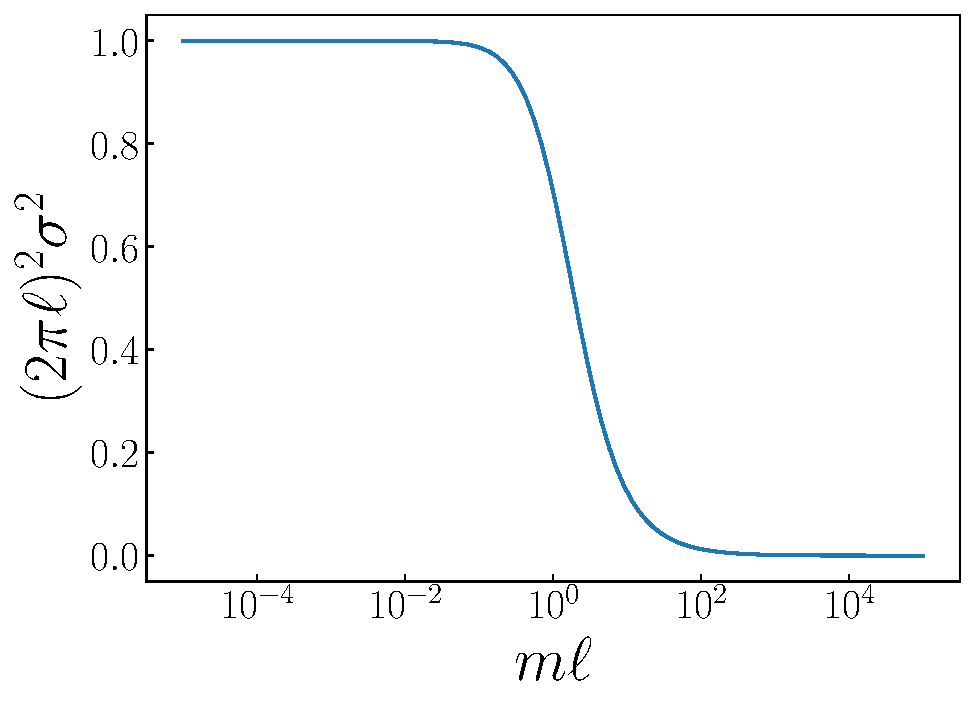
\includegraphics[width=0.7\textwidth]{prob4.pdf}
    \caption{Plot of $\sigma^2$, which is a measure of the zero-point fluctuations, as a function of $m \ell$.}
    \label{fig:prob4}
\end{figure}

}
    
\end{document}
